% begin module transformations-shifts
\begin{frame}
\frametitle{Transformations of Functions}
\begin{columns}[c]
\column{.5\textwidth}

\psset{xunit=1cm, yunit=1cm}
\begin{pspicture}(-5, -5)(5,5) 
\tiny 
\psframe*[linecolor=white](-5,-5)(5,5) 
\psaxes[ticks=none, labels=none]{<->}(0,0)(-0.5,-0.5)(4.5,4.5)
\rput[t](4.5, -0.1){$x$}
\rput[r](-0.1, 4.5){$y$}
%Function formula: 10/3+1/3 ((-3+3 (x))^{3})-1/3 ((-3+3 (x))^{2})-1/3 (x) 

\only<handout:0| -2>{
\psplot[linecolor=red, plotpoints=1000]{1.65}{2.55}{x -0.333333 mul x 3 mul -6 add 2 exp -0.333333 mul x 3 mul -6 add 3 exp 0.333333 mul 2.66667 add add add }
\rput[b] (2.55, 2.40654){\alert<-2>{$y=f(x)$}}
}
\only<handout:0| 3->{
\psplot[linecolor=blue, plotpoints=1000]{1.65}{2.55}{x -0.333333 mul x 3 mul -6 add 2 exp -0.333333 mul x 3 mul -6 add 3 exp 0.333333 mul 2.66667 add add add }
\rput[b] (2.55, 2.40654){$y=f(x)$}
}

\only<handout:0| 3>{%
\psplot[linecolor=red, plotpoints=1000]{1.65}{2.55}{x -0.333333 mul x 3 mul -6 add 2 exp -0.333333 mul x 3 mul -6 add 3 exp 0.333333 mul 4.16667 add add add }
\rput[b](2.55, 3.90654){\alert<3>{$y=f(x)+c$}}
}
\only<handout:0| 4->{%
\psplot[linecolor=blue, plotpoints=1000]{1.65}{2.55}{x -0.333333 mul x 3 mul -6 add 2 exp -0.333333 mul x 3 mul -6 add 3 exp 0.333333 mul 4.16667 add add add }
\rput[b](2.55, 3.90654){$y=f(x)+c$}
}


\only<handout:0| 4>{%
\psplot[linecolor=red, plotpoints=1000]{1.65}{2.55}{x -0.333333 mul x 3 mul -6 add 2 exp -0.333333 mul x 3 mul -6 add 3 exp 0.333333 mul 1.16667 add add add }
\rput[b](2.55, 0.906542){$y=f(x)-c$}
}
\only<handout:0| 5->{%
\psplot[linecolor=blue, plotpoints=1000]{1.65}{2.55}{x -0.333333 mul x 3 mul -6 add 2 exp -0.333333 mul x 3 mul -6 add 3 exp 0.333333 mul 1.16667 add add add }
\rput[b](2.55, 0.906542){$y=f(x)-c$}
}

\only<handout:0| 5>{%
\psplot[linecolor=red, plotpoints=1000]{3.15}{4.05}{x -0.333333 mul x 3 mul -10.5 add 2 exp -0.333333 mul x 3 mul -10.5 add 3 exp 0.333333 mul 3.16667 add add add }
\rput[b](4.05, 2.40654){\alert<5>{$y=f(x-c)$}}
}
\only<handout:0| 6->{%
\psplot[linecolor=blue, plotpoints=1000]{3.15}{4.05}{x -0.333333 mul x 3 mul -10.5 add 2 exp -0.333333 mul x 3 mul -10.5 add 3 exp 0.333333 mul 3.16667 add add add }
\rput[b](4.05, 2.40654){$y=f(x-c)$}
}

\only<6>{%
\psplot[linecolor=red, plotpoints=1000]{0.15}{1.05}{x -0.333333 mul x 3 mul -1.5 add 2 exp -0.333333 mul x 3 mul -1.5 add 3 exp 0.333333 mul 2.16667 add add add }
\rput[b](1.05, 2.40654){\alert<6>{$y=f(x+c)$}}
}
\end{pspicture} 
%\ \only<handout:0| -2>{%
%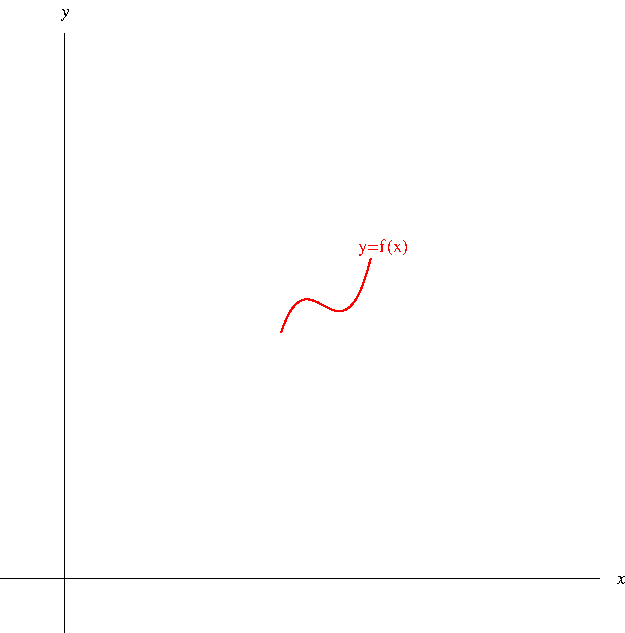
\includegraphics[height=5cm]{precalculus/pictures/01-03-shifta.pdf}%
%}%
%\only<handout:0| 3>{%
%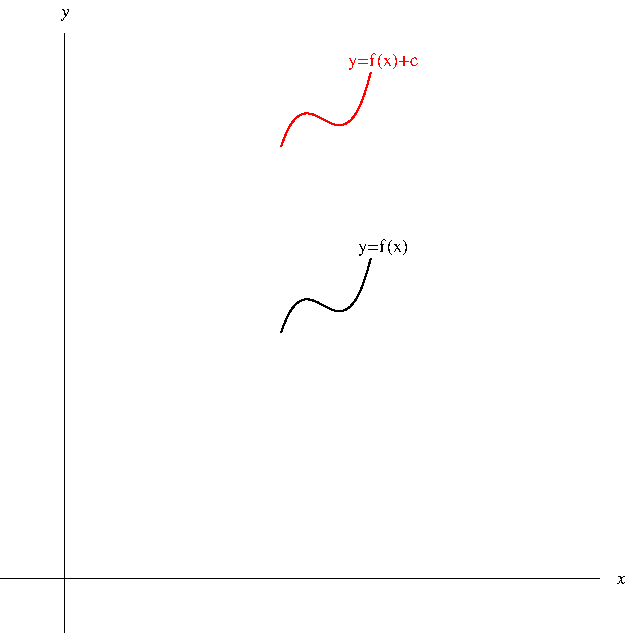
\includegraphics[height=5cm]{precalculus/pictures/01-03-shiftb.pdf}%
%}%
%\only<handout:0| 4>{%
%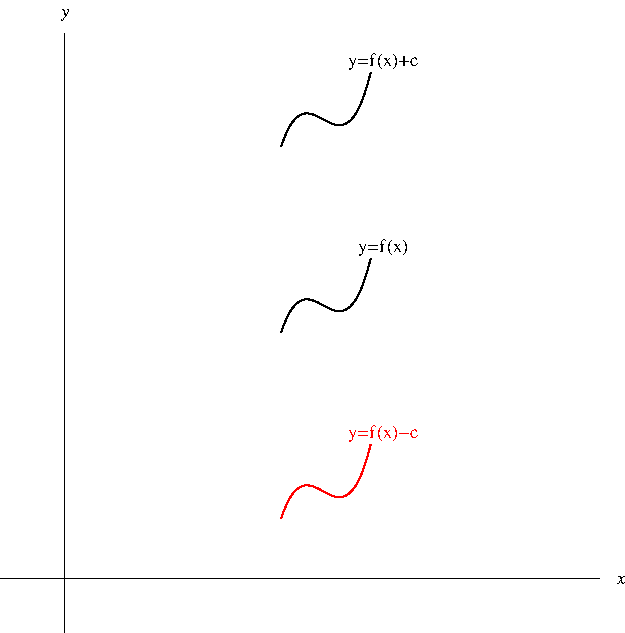
\includegraphics[height=5cm]{precalculus/pictures/01-03-shiftc.pdf}%
%}%
%\only<handout:0| 5>{%
%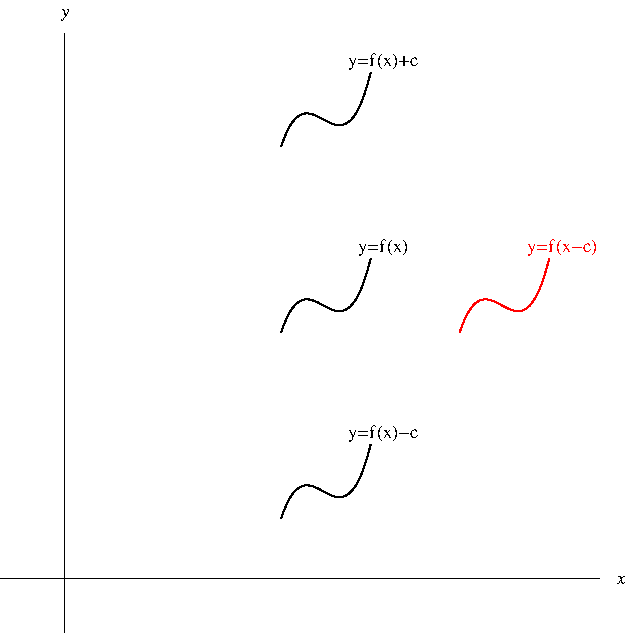
\includegraphics[height=5cm]{precalculus/pictures/01-03-shiftd.pdf}%
%}%
%\only<6>{%
%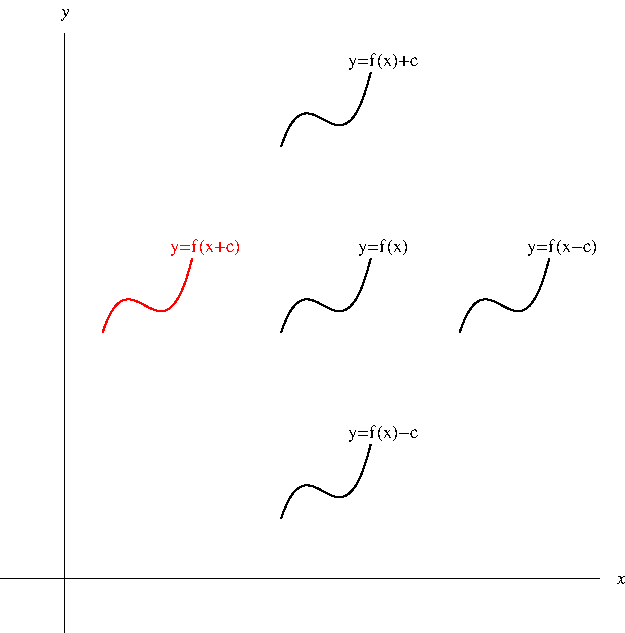
\includegraphics[height=5cm]{precalculus/pictures/01-03-shifte.pdf}%
%}%a
\column{.5\textwidth}
What happens if we add or subtract a positive constant $c$ in the equation of a function $f$?  What happens if we add or subtract $c$ from $x$ before applying the function $f$?
\end{columns}

\uncover<2->{
\begin{tabular}{|l|l|}
\hline
\alert<handout:0| 3>{$f(x)+c$} &%
\uncover<3->{\alert<handout:0| 3>{Shift the graph of $f(x)$ $c$ units up.}} \\%
\alert<handout:0| 4>{$f(x)-c$} &%
\uncover<4->{\alert<handout:0| 4>{Shift the graph of $f(x)$ $c$ units down.}} \\%
\alert<handout:0| 5>{$f(x-c)$} &%
\uncover<5->{\alert<handout:0| 5>{Shift the graph of $f(x)$ $c$ units right.}} \\%
\alert<handout:0| 6>{$f(x+c)$} &%
\uncover<6->{\alert<handout:0| 6>{Shift the graph of $f(x)$ $c$ units left.}}\\%
\hline
\end{tabular}
}
\end{frame}
% end module transformations-shifts